\documentclass[11pt,a4paper]{article}
\usepackage{amsmath, amsfonts, amssymb, amsthm}
\usepackage{tikz, pgfplots, tkz-euclide, calc}
    \usetikzlibrary{patterns, shapes.arrows, arrows.meta, calc}
\pgfplotsset{compat=1.18}
\allowdisplaybreaks[1]
\usepackage{fancyhdr}
\usepackage{enumerate, enumitem}
\usepackage{cancel}
\usepackage{varwidth}
\usepackage{hyperref}
\hypersetup{
    colorlinks=true,
    linkcolor=blue,
    filecolor=magenta,      
    urlcolor=cyan,
}

% TAMBAHKAN PACKAGE SENDIRI KALAU KURANG

\usepackage{geometry}
\geometry{
	left = 16mm,
	right = 16mm,
	top = 30mm,
	bottom = 30mm,
}

\setlength{\headheight}{16pt}
\pagestyle{fancy}
\fancyhead{}
\fancyfoot{}
\fancyhead[r]{}
\fancyhead[l]{\fbox{\large{\textbf{SKPB - ITS}}}}
\renewcommand{\headrulewidth}{0pt}
\renewcommand{\footrulewidth}{0pt}

\newcommand{\mulaisolusi}{%
    \clearpage
    \fancyhead{}
    \fancyhead[L]{\textit{Solution By: \href{https://github.com/TetewHeroez}{Tetew}}}
    \fancyfoot{}
    \renewcommand{\headrulewidth}{1pt}
    \renewcommand{\arraystretch}{1.5}
    \begin{center}\textbf{SOLUSI}\end{center}
}

\begin{document}

\fancyfoot[C]{%
  \hrulefill\textbf{ Have a great time doing it }\hrulefill
  \begin{center}``\textit{Honesty is the key to success}''\end{center}}

\begin{center}
  \underline{\textbf{\MakeUppercase{Quiz 1 Odd Semester 2026/2027}}}
\end{center}

\begin{center}
  \begin{tabular}{lcl}
    Course/Credits  & : & Calculus 1 / 3 SKS            \\
    Day, Date       & : & Tuesday, 17 November 2026     \\
    Time (Duration) & : & 15.30-17.10 WIB (100 minutes) \\
    Properties      & : & Closed book                   \\
    Class           & : & 64
  \end{tabular}
\end{center}

\noindent\rule{\textwidth}{2pt}
\vspace*{-0.9cm}
\begin{center}
  Five questions are provided, along with the weight for each question.\\
  Write your name, student ID number (NRP), and class number on your answer sheet.\\
  {\textbf{\MakeUppercase{Calculators and communication devices are prohibited.}}\\
    \textbf{\MakeUppercase{Giving or receiving answers during the exam is prohibited.}}}\\
  \textbf{``Any act of dishonesty will result in academic sanctions.''}
\end{center}
\vspace*{-0.5cm}
\noindent\rule{\textwidth}{2pt}

\begin{enumerate}
  \item (Weight 25) Let $l$ be the length of the diagonal of a rectangle with sides $x$ and $y$, and assume that $x$ and $y$ are functions of time.
        \begin{enumerate}
          \item What is the relationship between $\dfrac{dl}{dt}$, $\dfrac{dx}{dt}$, and $\dfrac{dy}{dt}$?
          \item At a certain instant, $x$ is increasing at a rate of 1/2 cm/sec, and $y$ is decreasing at a rate of 1/4 cm/sec. How fast is the length of the diagonal changing when $x = 3\text{ cm}$ and $y = 4\text{ cm}$? Is the diagonal increasing or decreasing at that moment?
        \end{enumerate}

  \item (Weight 50) Given $y = \dfrac{x^2}{x^2 - 1}$.
        \begin{enumerate}
          \item Determine the $x$-intercept(s), if any.
          \item Determine the $y$-intercept(s), if any.
          \item Determine the vertical asymptote(s).
          \item Determine the horizontal asymptote(s).
          \item Determine the first derivative.
          \item Determine the intervals of increase and decrease.
          \item Determine the second derivative.
          \item Determine the intervals of concavity (concave up and concave down).
          \item Sketch the graph of the function.
        \end{enumerate}

  \item (Weight 25) Express the number 10 as the sum of two non-negative numbers whose product is as large as possible.
\end{enumerate}

\mulaisolusi
\begin{enumerate}
  \item Look at the following image
        \begin{center}
          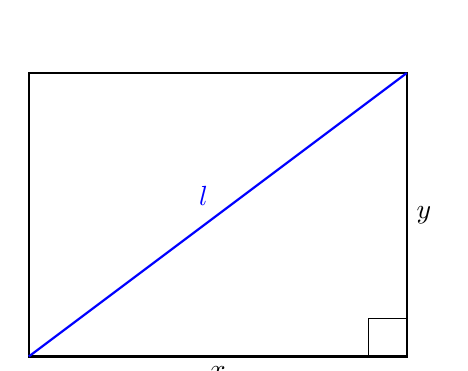
\begin{tikzpicture}[scale=1.2]
            % Rectangle
            \draw[thick] (0,0) rectangle (4,3);
            % Diagonal
            \draw[thick, blue] (0,0) -- (4,3);
            % Labels
            \node[below] at (2,0) {$x$};
            \node[right] at (4,1.5) {$y$};
            \node[above left, blue] at (2,1.5) {$l$};
            % Right angle symbol
            \draw (3.6,0) -- (3.6,0.4) -- (4,0.4);
          \end{tikzpicture}
        \end{center}
        \begin{enumerate}
          \item Based on the Pythagorean theorem, the length of the diagonal $l$ is related to the sides $x$ and $y$ by:
                \[
                  l^2 = x^2 + y^2
                \]
                Since $x$, $y$, and $l$ are functions of time $t$, we differentiate both sides implicitly with respect to $t$:
                \begin{align*}
                  \frac{d}{dt}\left(l^2\right) & = \frac{d}{dt}\left(x^2 + y^2\right) \\
                  2l\frac{dl}{dt}              & = 2x\frac{dx}{dt} + 2y\frac{dy}{dt}
                \end{align*}
                Dividing both sides by $2$:
                \[
                  l\frac{dl}{dt} = x\frac{dx}{dt} + y\frac{dy}{dt}
                \]
                Since $l = \sqrt{x^2 + y^2} > 0$, the relationship between $\dfrac{dl}{dt}$, $\dfrac{dx}{dt}$, and $\dfrac{dy}{dt}$ is:
                \[
                  \boxed{\frac{dl}{dt} = \frac{x\dfrac{dx}{dt} + y\dfrac{dy}{dt}}{l} = \frac{x\dfrac{dx}{dt} + y\dfrac{dy}{dt}}{\sqrt{x^2 + y^2}}}
                \]

          \item From the problem description, we are given:
                \begin{itemize}
                  \item $\dfrac{dx}{dt} = \dfrac{1}{2}\text{ cm/sec}$ ($x$ is increasing)
                  \item $\dfrac{dy}{dt} = -\dfrac{1}{4}\text{ cm/sec}$ ($y$ is decreasing)
                  \item At the given instant: $x = 3\text{ cm}$ and $y = 4\text{ cm}$
                \end{itemize}
                First, calculate the length of the diagonal $l$ at this instant:
                \[
                  l = \sqrt{x^2 + y^2} = \sqrt{3^2 + 4^2} = \sqrt{9 + 16} = \sqrt{25} = 5\text{ cm}.
                \]
                Substituting these values into the rate equation obtained in part (a):
                \begin{align*}
                  \frac{dl}{dt} & = \frac{x\dfrac{dx}{dt} + y\dfrac{dy}{dt}}{l}                                      \\
                                & = \frac{3\left(\dfrac{1}{2}\right) + 4\left(-\dfrac{1}{4}\right)}{5}               \\
                                & = \frac{\dfrac{3}{2} - 1}{5}                                                       \\
                                & = \frac{\dfrac{1}{2}}{5} = \boxed{\frac{1}{10}\text{ cm/sec} = 0.1\text{ cm/sec}}.
                \end{align*}
                Since $\dfrac{dl}{dt} = \dfrac{1}{10} > 0$, the length of the diagonal is \textbf{increasing} at a rate of $\boxed{\dfrac{1}{10}\text{ cm/sec}}$ (or $0.1\text{ cm/sec}$).
        \end{enumerate}

  \item Given the rational function:
        \[
          y = f(x) = \frac{x^2}{x^2 - 1}
        \]
        The domain of $f$ is all real numbers except where $x^2 - 1 = 0$, so $\mathcal{D}_f = \mathbb{R} \setminus \{-1, 1\} = (-\infty, -1) \cup (-1, 1) \cup (1, \infty)$.

        \begin{enumerate}
          \item \textbf{$x$-intercept(s):}\\
                The $x$-intercept occurs when $y = 0$:
                \[
                  \frac{x^2}{x^2 - 1} = 0 \implies x^2 = 0 \implies x = 0.
                \]
                Since $x = 0$ is in the domain, the $x$-intercept is at $\boxed{(0, 0)}$.

          \item \textbf{$y$-intercept(s):}\\
                The $y$-intercept occurs when $x = 0$:
                \[
                  y = f(0) = \frac{0^2}{0^2 - 1} = 0.
                \]
                Thus, the $y$-intercept is at $\boxed{(0, 0)}$.

          \item \textbf{Vertical asymptote(s):}\\
                Vertical asymptotes occur at the zeros of the denominator that do not cancel with the numerator:
                \[
                  x^2 - 1 = 0 \implies (x - 1)(x + 1) = 0 \implies x = 1 \quad\text{or}\quad x = -1.
                \]
                Evaluating the one-sided limits:
                \begin{align*}
                  \lim_{x \to 1^+} \frac{x^2}{x^2 - 1}  & = +\infty, \qquad \lim_{x \to 1^-} \frac{x^2}{x^2 - 1} = -\infty,  \\
                  \lim_{x \to -1^+} \frac{x^2}{x^2 - 1} & = -\infty, \qquad \lim_{x \to -1^-} \frac{x^2}{x^2 - 1} = +\infty.
                \end{align*}
                Therefore, the vertical asymptotes are $\boxed{x = -1}$ and $\boxed{x = 1}$.

          \item \textbf{Horizontal asymptote(s):}\\
                We evaluate the limits as $x \to \pm\infty$:
                \[
                  \lim_{x \to \infty} \frac{x^2}{x^2 - 1} = \lim_{x \to \infty} \frac{1}{1 - \frac{1}{x^2}} = 1,
                \]
                \[
                  \lim_{x \to -\infty} \frac{x^2}{x^2 - 1} = \lim_{x \to -\infty} \frac{1}{1 - \frac{1}{x^2}} = 1.
                \]
                Therefore, the horizontal asymptote is $\boxed{y = 1}$.

          \item \textbf{First derivative:}\\
                Using the quotient rule $\left(\dfrac{u}{v}\right)' = \dfrac{u'v - uv'}{v^2}$ with $u = x^2$ and $v = x^2 - 1$:
                \begin{align*}
                  f'(x) & = \frac{\frac{d}{dx}(x^2)\cdot(x^2 - 1) - x^2\cdot\frac{d}{dx}(x^2 - 1)}{(x^2 - 1)^2} \\
                        & = \frac{2x(x^2 - 1) - x^2(2x)}{(x^2 - 1)^2}                                           \\
                        & = \frac{2x^3 - 2x - 2x^3}{(x^2 - 1)^2}                                                \\
                        & = \boxed{-\frac{2x}{(x^2 - 1)^2}}.
                \end{align*}

          \item \textbf{Intervals of increase and decrease:}\\
                The critical numbers occur where $f'(x) = 0$ or where $f'(x)$ is undefined:
                \begin{itemize}
                  \item $f'(x) = 0 \iff -2x = 0 \iff x = 0$.
                  \item $f'(x)$ is undefined at $x = \pm 1$ (which are vertical asymptotes, not in the domain).
                \end{itemize}
                Since the denominator $(x^2 - 1)^2 > 0$ for all $x \in \mathcal{D}_f$, the sign of $f'(x)$ is determined solely by $-2x$:
                \[
                  \begin{array}{c|cccc}
                    \text{Interval}       & (-\infty, -1)     & (-1, 0)           & (0, 1)            & (1, +\infty)      \\ \hline
                    \text{Sign of } f'(x) & +                 & +                 & -                 & -                 \\
                    \text{Behavior}       & \text{Increasing} & \text{Increasing} & \text{Decreasing} & \text{Decreasing}
                  \end{array}
                \]
                Therefore:
                \begin{itemize}
                  \item $f(x)$ is \textbf{increasing} on $\boxed{(-\infty, -1)}$ and $\boxed{(-1, 0]}$ (or $(-\infty, -1) \cup (-1, 0)$).
                  \item $f(x)$ is \textbf{decreasing} on $\boxed{[0, 1)}$ and $\boxed{(1, +\infty)}$ (or $(0, 1) \cup (1, +\infty)$).
                \end{itemize}
                (\textit{Note}: By the First Derivative Test, there is a local maximum at $(0, f(0)) = (0, 0)$).

          \item \textbf{Second derivative:}\\
                Differentiating $f'(x) = \dfrac{-2x}{(x^2 - 1)^2}$ using the quotient rule:
                \begin{align*}
                  f''(x) & = \frac{\frac{d}{dx}(-2x)\cdot(x^2 - 1)^2 - (-2x)\cdot\frac{d}{dx}\left((x^2 - 1)^2\right)}{\left((x^2 - 1)^2\right)^2} \\
                         & = \frac{-2(x^2 - 1)^2 - (-2x)\left[2(x^2 - 1)(2x)\right]}{(x^2 - 1)^4}                                                  \\
                         & = \frac{(x^2 - 1)\left[-2(x^2 - 1) + 8x^2\right]}{(x^2 - 1)^4}                                                          \\
                         & = \frac{-2x^2 + 2 + 8x^2}{(x^2 - 1)^3}                                                                                  \\
                         & = \boxed{\frac{6x^2 + 2}{(x^2 - 1)^3} = \frac{2(3x^2 + 1)}{(x^2 - 1)^3}}.
                \end{align*}

          \item \textbf{Intervals of concavity:}\\
                Notice that the numerator $2(3x^2 + 1) \ge 2 > 0$ for all $x \in \mathbb{R}$. Thus, the sign of $f''(x)$ is completely determined by the sign of $(x^2 - 1)^3$, which is identical to the sign of $x^2 - 1$:
                \[
                  \begin{array}{c|ccc}
                    \text{Interval}        & (-\infty, -1)             & (-1, 1)                     & (1, +\infty)              \\ \hline
                    \text{Sign of } f''(x) & +                         & -                           & +                         \\
                    \text{Concavity}       & \text{Concave Up } (\cup) & \text{Concave Down } (\cap) & \text{Concave Up } (\cup)
                  \end{array}
                \]
                Therefore:
                \begin{itemize}
                  \item $f(x)$ is \textbf{concave up} on $\boxed{(-\infty, -1) \cup (1, +\infty)}$.
                  \item $f(x)$ is \textbf{concave down} on $\boxed{(-1, 1)}$.
                \end{itemize}
                Since $f''(x) \ne 0$ everywhere and $x = \pm 1$ are not in the domain, there are \textbf{no inflection points}.

          \item \textbf{Sketch of the graph:}\\
                Combining the above properties:
                \begin{itemize}
                  \item The graph has a local maximum at $(0, 0)$.
                  \item Vertical asymptotes at $x = -1$ and $x = 1$.
                  \item Horizontal asymptote at $y = 1$.
                  \item Symmetry: $f(-x) = \dfrac{(-x)^2}{(-x)^2 - 1} = \dfrac{x^2}{x^2 - 1} = f(x)$, so the function is even and symmetric about the $y$-axis.
                \end{itemize}
                \begin{center}
                  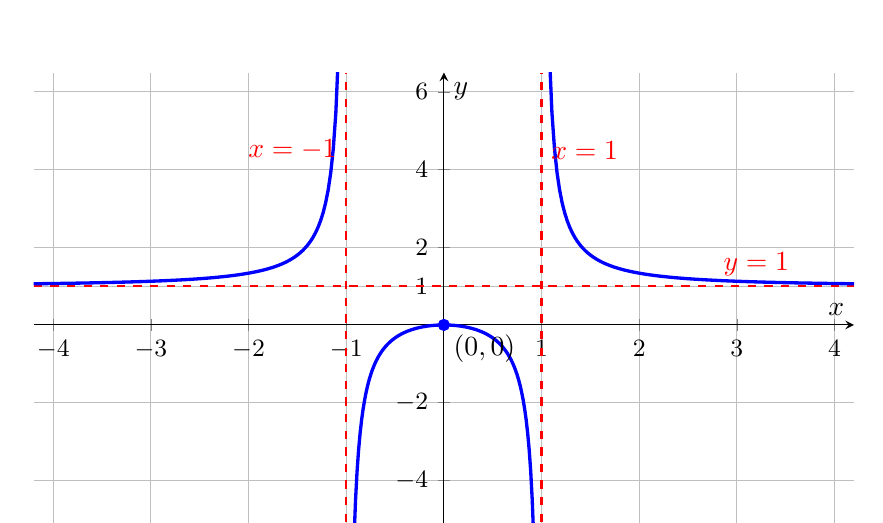
\begin{tikzpicture}
                    \begin{axis}[
                        width=12cm, height=7.5cm,
                        axis lines=middle,
                        xmin=-4.2, xmax=4.2,
                        ymin=-5.5, ymax=6.5,
                        xlabel=$x$, ylabel=$y$,
                        grid=major,
                        xtick={-4,-3,-2,-1,0,1,2,3,4},
                        ytick={-4,-2,0,1,2,4,6},
                        ticklabel style={font=\small},
                        restrict y to domain=-7:8,
                        unbounded coords=discard
                      ]
                      % Asymptotes
                      \addplot[dashed, red, thick] coordinates {(-1,-5.5) (-1,6.5)};
                      \addplot[dashed, red, thick] coordinates {(1,-5.5) (1,6.5)};
                      \addplot[dashed, red, thick, domain=-4.2:4.2] {1};

                      % Curve branches
                      \addplot[blue, very thick, domain=-4.2:-1.08, samples=120] {x^2/(x^2-1)};
                      \addplot[blue, very thick, domain=-0.92:0.92, samples=120] {x^2/(x^2-1)};
                      \addplot[blue, very thick, domain=1.08:4.2, samples=120] {x^2/(x^2-1)};

                      % Key Points
                      \addplot[only marks, mark=*, mark size=2pt, color=blue] coordinates {(0,0)};
                      \node[below right] at (axis cs:0,0) {$(0,0)$};

                      % Labels for asymptotes
                      \node[above, red] at (axis cs:3.2, 1) {$y = 1$};
                      \node[left, red] at (axis cs:-1, 4.5) {$x = -1$};
                      \node[right, red] at (axis cs:1, 4.5) {$x = 1$};
                    \end{axis}
                  \end{tikzpicture}
                \end{center}
        \end{enumerate}

        \newpage
  \item \textbf{Optimization (Optimasi)}

        Let the two non-negative numbers be $x$ and $y$, so:
        \[
          x \ge 0 \quad\text{and}\quad y \ge 0.
        \]
        The sum of the two numbers is given as $10$:
        \[
          x + y = 10 \implies y = 10 - x.
        \]
        Since $y \ge 0$, we have $10 - x \ge 0 \implies x \le 10$. Therefore, $x$ is restricted to the closed interval:
        \[
          x \in [0, 10].
        \]
        We want to maximize their product, denoted by $P(x)$:
        \[
          P(x) = x \cdot y = x(10 - x) = 10x - x^2.
        \]
        To find the absolute maximum of $P(x)$ on $[0, 10]$, we first find the critical numbers by setting the first derivative equal to zero:
        \[
          P'(x) = \frac{d}{dx}(10x - x^2) = 10 - 2x.
        \]
        Setting $P'(x) = 0$:
        \[
          10 - 2x = 0 \implies 2x = 10 \implies x = 5.
        \]
        Since $x = 5$ lies in the interval $[0, 10]$, it is a valid critical point.

        \textbf{Testing for Maximum:}
        \begin{itemize}
          \item \textbf{Second Derivative Test:}
                \[
                  P''(x) = -2 < 0 \quad \text{for all } x.
                \]
                Since $P''(5) = -2 < 0$, the function $P(x)$ is strictly concave down everywhere, which confirms that $x = 5$ gives a unique global maximum.
          \item \textbf{Closed Interval Method (Endpoint Evaluation):}
                \begin{align*}
                  P(0)  & = 0(10 - 0) = 0,   \\
                  P(5)  & = 5(10 - 5) = 25,  \\
                  P(10) & = 10(10 - 10) = 0.
                \end{align*}
                The maximum product value is $25$, occurring at $x = 5$.
        \end{itemize}

        Substituting $x = 5$ into the expression for $y$:
        \[
          y = 10 - 5 = 5.
        \]
        Both numbers are non-negative ($5 \ge 0$).

        Thus, the two non-negative numbers whose sum is $10$ and whose product is as large as possible are:
        \[
          \boxed{5 \quad\text{and}\quad 5}.
        \]

        \medskip
        \noindent\textit{Alternative Method (AM-GM Inequality):}\\
        For any non-negative real numbers $x, y \ge 0$, by the Arithmetic Mean--Geometric Mean (AM--GM) inequality:
        \[
          \sqrt{xy} \le \frac{x + y}{2} = \frac{10}{2} = 5.
        \]
        Squaring both sides:
        \[
          xy \le 25.
        \]
        Equality holds if and only if $x = y$. Since $x + y = 10$, this immediately yields $x = y = 5$.
\end{enumerate}

\end{document}
